\chapter{双图理论：认知结构图与功能拓扑图}

\begin{chapteroverviewbox}
在前一章中，我们已经把智能体从传统的“模块集合”重新定义为一个由功能节点、功能关系与多尺度闭环组成的动态功能拓扑。然而，仅有功能拓扑仍然不足以描述智能。功能拓扑能够告诉我们“系统有哪些处理能力、这些能力怎样相互作用”，却不能回答另一个同样根本的问题：\textbf{系统此刻究竟在处理什么结构，这些认知结构之间存在怎样的语义、因果、时间、目标与自指关系？}

为此，本章正式引入“双图理论”（Dual-Graph Theory）。我们把一个持续智能体同时描述为两张彼此耦合、但本体上不可混同的动态图：第一张是认知结构图
\[
\mathcal G_C,
\]
它描述CSO及其关系；第二张是功能拓扑图
\[
\mathcal G_F,
\]
它描述智能系统中具有因果作用的功能节点、功能连接与闭环。二者之间通过随时间变化的承载映射
\[
\mu_t:\mathcal G_C\rightarrow\mathcal G_F
\]
发生耦合。

这一分离使我们第一次可以严格区分：\textbf{“智能正在思考什么”与“这些认知结构现在由什么功能承载和处理”}。它也是后续CSO迁移、技能形成、记忆沉降、认知卸载、功能拓扑学习以及AgentOS结构发育理论的数学基础。

本章的核心命题可以浓缩为：
\begin{statementbox}
\centering
\adjustbox{max width=.96\linewidth}{\(\displaystyle \text{智能动力学}
=
\text{认知结构动力学}
\bowtie
\text{功能承载动力学}\)}
\end{statementbox}
或者更加简洁地写成：
\[
\boxed{
Dynamics\ On\ Topology
+
Dynamics\ Of\ Topology
}
\]

需要特别说明的是，本章借用了图论、多层网络、超图、动态网络、双部图、图映射以及控制系统中的状态--实现分离思想，但“双图理论”在本书中的具体含义，是为CSO、Agent-CSO及AgentOS长期智能动力学服务的理论构造，不应与任何一种现成图神经网络或知识图谱模型直接等同。
\end{chapteroverviewbox}

\begin{figure}[htbp]
\centering
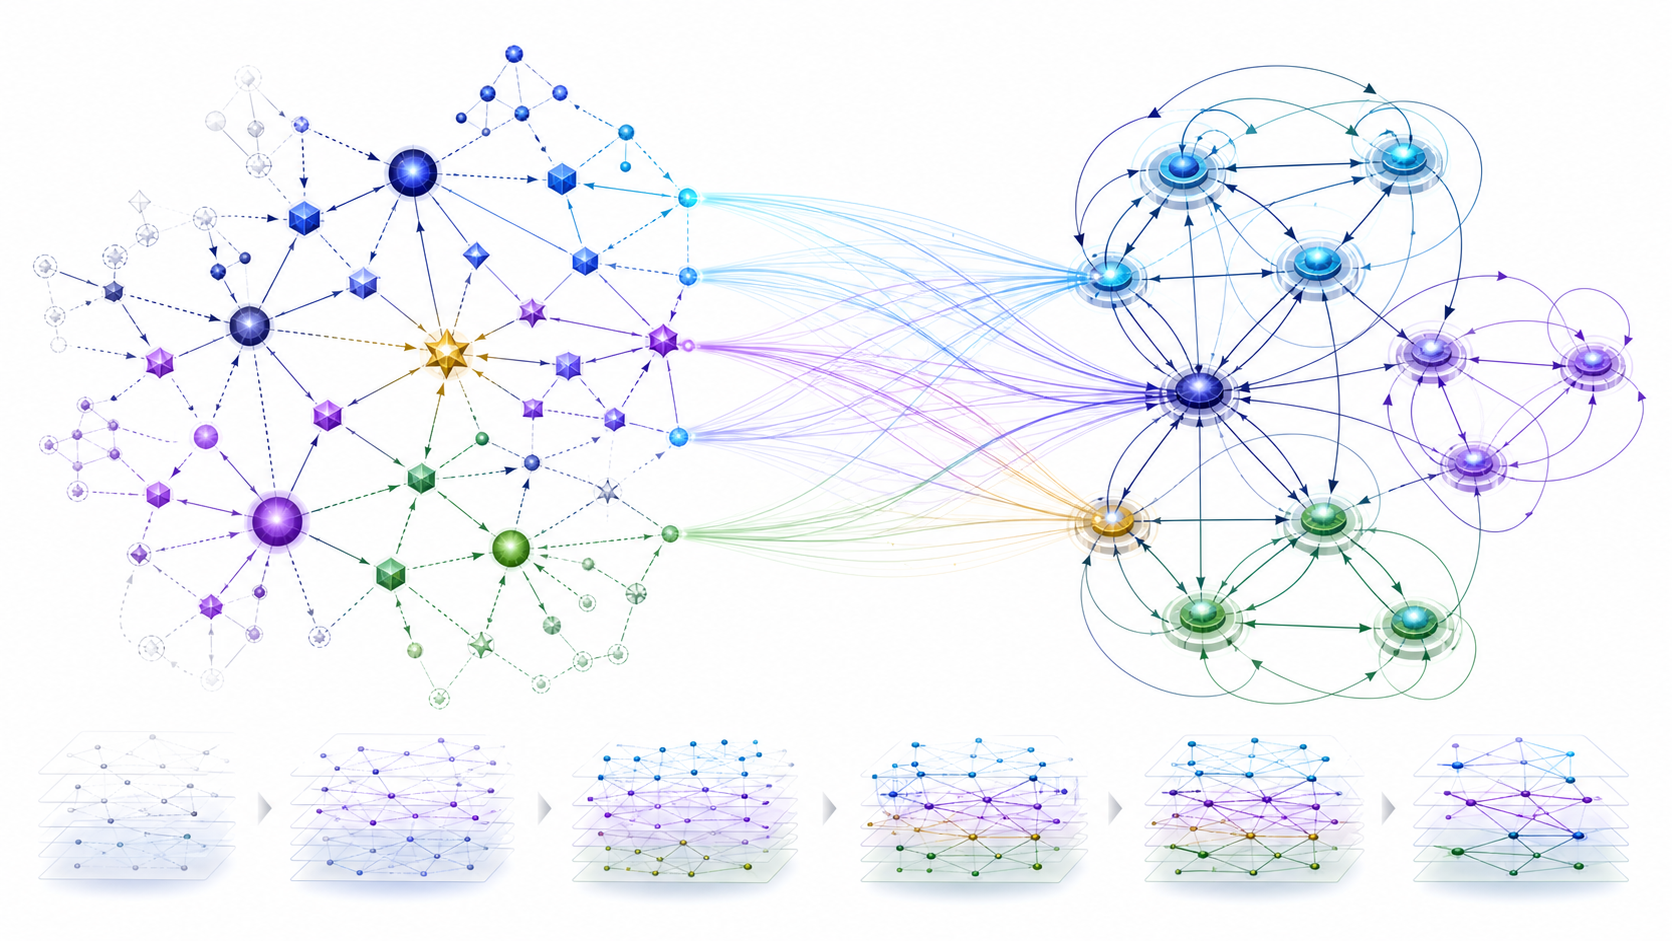
\includegraphics[width=.9\textwidth,height=.38\textheight,keepaspectratio]{images/cognitive-structure-functional-topology.png}
\caption{CSO 图、功能图与多对多承载映射}
\end{figure}
\section{为什么一张图不足以描述智能}

在构造智能理论时，一个极易出现的错误，是试图用同一张结构图同时表示“世界中的认知对象”和“处理这些对象的系统结构”。这种做法在简单系统中并不会立刻暴露问题。例如，我们可以画出“视觉模块$\rightarrow$规划模块$\rightarrow$动作模块”，并在每个模块内部附上当前处理的信息，看上去似乎已经完整描述了智能过程。然而，一旦系统进入持续学习、多尺度记忆、技能迁移、外部工具使用以及长期身份连续的场景，这种表示很快失效。

原因在于，认知内容与功能承载并不是一一绑定的。

例如，一个具体的空间关系CSO
\[
C_{\text{cup-on-table}}
\]
在刚刚被感知时，可能主要由感知整合功能承载；在进入工作记忆以后，它可能被规划、语言推理和目标评估同时调用；在经验沉降之后，它可能进入情景记忆；若该结构长期重复出现，则其中某部分甚至可能被编译进身体控制技能，使其不再需要显式进入工作记忆。换言之，同一个认知结构可以沿着不同功能和不同时间尺度发生迁移。

因此，如果我们把认知对象直接等同于功能模块内部状态，就会隐含一个错误假设：
\[
\boxed{
CognitiveStructure
\equiv
FunctionalLocation
}
\]
而长期智能恰恰要求我们否定这一等同。

更加准确的关系应当是：
\[
\boxed{
CognitiveStructure
\neq
FunctionalCarrier
}
\]
但同时：
\begin{statementbox}
\centering
\adjustbox{max width=.96\linewidth}{\(\displaystyle CognitiveStructure
\ \text{必须在某个时刻由某种功能结构实现}\)}
\end{statementbox}

这正是双图理论的起点。

我们可以用一个简单例子说明。假设智能体正在学习“打开某种陌生门锁”。最初，与门锁有关的CSO包括把手位置、旋转方向、阻力、按钮状态、视觉纹理、动作结果等。这些认知结构之间本身已经形成一张关系图：
\[
\mathcal G_C.
\]
与此同时，智能体内部存在视觉整合、空间表征、工作记忆、规划、动作控制、残差检测、经验写入等功能，它们形成另一张图：
\[
\mathcal G_F.
\]

在第一次尝试时，门锁结构可能经历：
\[
Perception
\rightarrow
h
\rightarrow
Planning
\rightarrow
MotorControl.
\]

第几十次以后，同样的结构可能变为：
\[
Perception
\rightarrow
BodySkill.
\]

外部世界中的问题没有发生本体上的根本改变，但Agent内部的承载方式已经发生重大改变。因此，真正的学习不能只表示为某个模块内部参数变化，而必须允许：
\begin{statementbox}
\centering
\adjustbox{max width=.96\linewidth}{\(\displaystyle CSO@F_i
\rightarrow
CSO@F_j\)}
\end{statementbox}

这里的“@”并不是空间位置符号，而表示“某一认知结构当前主要由某一功能结构承载、激活、转换或控制”。

双图理论因而把智能系统拆成两个不同的问题。第一类问题是：
\[
\text{What cognitive structure exists?}
\]
即认知结构之间如何形成关系、变化和组合。第二类问题是：
\[
\text{Where and how is that structure functionally carried?}
\]
即这些结构由何种功能、何种时间尺度以及何种内部或外部载体承担。

从理论方法上看，这种分离类似于计算机科学中“程序语义”与“运行实现”的区分，也类似于控制理论中“任务空间”和“状态实现空间”的区分，还可以与多层网络理论中的不同关系层进行比较。但这些外部理论只能提供形式上的帮助。本书中的根本对象仍然是CSO及其动态承载，而不是传统的数据节点或静态网络实体。

因此，本章建立的第一条原则是：
\begin{proposition*}
\bfseries 认知关系结构与实现这些关系的功能结构必须分层描述。
\end{proposition*}

只有完成这一分离，我们才能进一步讨论为什么一个智能体能够在保持“知道同一件事”的同时，逐渐改变自己“怎样知道、在哪里知道以及需要多少显式认知才能知道”。

\section{认知结构图：$\mathcal G_C$}

我们首先定义认知结构图。设一个Agent在时刻$t$能够形成或保持的有效CSO集合为
\[
V_C(t)=\{C_1,C_2,\ldots,C_{N_C(t)}\}.
\]
这里每个$C_i$并不等于一个token、一个向量或一个固定的数据库实体，而表示一个在当前理论尺度上具有独立结构意义的认知结构对象。它可以是对象、事件、关系、规则、目标、约束、因果结构、动作模式、自我状态、价值判断或未来可能性。

这些CSO之间通过不同类型的关系连接。于是我们定义：
\[
\boxed{
\mathcal G_C(t)
=
\left(
V_C(t),
E_C(t),
\Lambda_C
\right)
}
\]
其中$V_C$是CSO集合，$E_C$是关系集合，$\Lambda_C$则定义允许存在的关系类型空间。

需要强调，认知结构图通常不是一个简单无向图。对于长期智能而言，至少应允许以下几类关系：
\[
\Lambda_C
=
\{
R_{\text{semantic}},
R_{\text{causal}},
R_{\text{temporal}},
R_{\text{spatial}},
R_{\text{goal}},
R_{\text{constraint}},
R_{\text{predictive}},
R_{\text{self}},
R_{\text{value}}
\}.
\]

例如：
\[
C_A
\xrightarrow{R_{\text{causal}}}
C_B
\]
表示智能体认为$A$在某种意义上导致$B$；
而
\[
C_G
\xrightarrow{R_{\text{constraint}}}
C_P
\]
可以表示目标CSO对规划CSO施加约束。

因此$\mathcal G_C$更加接近一种有类型、有方向、有时间属性的多关系图。更加一般地，可以写成：
\[
E_C(t)
\subseteq
V_C(t)
\times
\Lambda_C
\times
V_C(t).
\]

然而，即使这一形式仍然可能不足。现实认知经常出现一个关系同时依赖多个结构的情况。例如，“如果门锁处于锁定状态并且钥匙已经插入，那么顺时针旋转可以打开门”并不是简单二元关系，而可以表示为：
\[
\{C_{\text{locked}},C_{\text{key-in}}\}
\rightarrow
C_{\text{rotate-clockwise}}
\rightarrow
C_{\text{open}}.
\]
因此，在更严格的实现中，$\mathcal G_C$更适合推广为有类型超图：
\[
\boxed{
\mathcal H_C
=
(V_C,\mathcal E_C)
}
\]
其中每一个超边可以连接多个CSO。

从动力学角度看，$\mathcal G_C$也不是静态知识库。它随时间发生至少五类变化。

第一类是CSO生成：
\[
C_{\text{new}}\notin V_C(t),
\qquad
C_{\text{new}}\in V_C(t+\Delta t).
\]

第二类是关系生成：
\[
e_{ij}:0\rightarrow1.
\]

第三类是关系权重变化：
\[
w_{ij}^C(t)
\rightarrow
w_{ij}^C(t+\Delta t).
\]

第四类是CSO合并或抽象，例如多个具体经验：
\[
C_1,C_2,\ldots,C_n
\]
经过结构化学习后，形成更高层结构：
\[
C_\Theta
=
\Phi(C_1,\ldots,C_n).
\]

第五类是遗忘、失活或降阶。一些CSO并不是完全消失，而是从当前可直接访问的图结构中退出，成为潜在结构或被压缩进更高层生成器。

因此，认知结构图的真正动力学可以写成：
\[
\boxed{
\dot{\mathcal G}_C
=
F_C
\left(
\mathcal G_C,
O_t,
A_t,
\mathcal G_F,
M_t
\right)
}
\]
其中$O_t$表示观察输入，$A_t$表示行动及其现实反馈，$\mathcal G_F$表示当前功能承载结构，$M_t$表示记忆、多尺度状态和自我约束。

这里有一个关键点：$\mathcal G_C$并不是“客观世界本身”。它是智能体内部对世界、自身和未来可能性的结构化认知，因此严格来说，进入Agent内部以后，更接近Agent-CSO图。后续如果需要区分宇宙本体CSO与Agent内部承载，我们可以进一步写：
\[
\mathcal G_U
\xrightarrow{O_A}
\mathcal G_C^A.
\]
其中$\mathcal G_U$是现实结构图，而$\mathcal G_C^A$是Agent $A$形成的认知结构图。

因此，两个不同Agent面对同一现实：
\[
\mathcal G_U
\]
可能得到：
\[
\mathcal G_C^A
\neq
\mathcal G_C^B.
\]
这并不是理论缺陷，而正是Agent特异性、经验差异与身体差异的来源。

从外部理论来看，知识图谱、语义网络、frame semantics、schema theory、causal graph以及world model都提供了与$\mathcal G_C$相关的研究工具。但本书并不把$\mathcal G_C$限制为“显式知识图谱”。其节点既可以具有符号接口，也可以由分布式潜变量实现；真正重要的是这些不同实现是否能够保持相同的主要结构关系和功能作用。

因此，本节的核心结论是：
\begin{conclusion}
\bfseries
$\mathcal G_C$描述的是智能体认知世界中的结构关系，而不是承载这些结构的处理器位置。
\end{conclusion}

它回答的是“什么结构存在、这些结构之间如何关联”。至于“谁在处理它们”，必须交给第二张图。

\section{功能拓扑图：$\mathcal G_F$}

与认知结构图不同，功能拓扑图描述的是智能系统本身的因果处理组织。设智能体拥有一组能够对Agent-CSO执行某种稳定变换的功能：
\[
V_F
=
\{
F_1,F_2,\ldots,F_{N_F}
\}.
\]
这里的$F_i$不是简单的软件模块名称，而是一个具有可区分输入、状态、输出和因果作用的功能单元。

例如，在AgentOS中，我们可以识别出：
\[
F_{\text{SPC}},
F_{\text{TCE}},
F_{\text{CCM}},
F_h,
F_E,
F_\Theta,
F_{\text{Scheduler}},
F_{\text{Boundary}},
F_{\text{Body}}
\]
等功能结构。但需要再次强调：本章的功能拓扑理论先于具体AgentOS模块。换一种实现，同样的功能关系完全可能由不同的软件、神经网络或硬件结构实现。

定义：
\[
\boxed{
\mathcal G_F(t)
=
\left(
V_F(t),
E_F(t),
\mathcal L_F(t),
W_F(t)
\right)
}
\]
其中：
\[
V_F
\]
是功能节点，
\[
E_F
\]
是功能耦合边，
\[
\mathcal L_F
\]
是闭环集合，
\[
W_F
\]
表示边的强度、时延、带宽、权限或其他运行参数。

与传统模块图相比，加入$\mathcal L_F$非常重要。因为智能并不是简单的数据流水线，而是多闭环系统。例如：
\[
F_{\text{SPC}}
\rightarrow
F_{\text{TCE}}
\rightarrow
F_h
\rightarrow
F_{\text{SPC}}
\]
就是一个认知控制闭环；而：
\[
F_h
\rightarrow
F_E
\rightarrow
F_\Theta
\rightarrow
F_h
\]
又形成记忆结构循环。

同一个功能节点可以同时属于多个闭环：
\[
F_i
\in
L_a\cap L_b\cap L_c.
\]
这也是为什么在理论上采用超图或闭环集合比传统树状模块图更合适。

每一个功能节点可以抽象成一个状态转移算子：
\[
x_i(t+\Delta t)
=
\Phi_i
\left(
x_i(t),
I_i(t),
u_i(t)
\right),
\]
其中$x_i$是节点内部状态，$I_i$是从其他功能节点或现实世界进入的输入，$u_i$是高层控制或边界约束。

如果更强调CSO的处理，可以定义：
\[
\boxed{
F_i:
\mathcal C_A
\rightarrow
\mathcal C_A
}
\]
即功能节点将一组Agent-CSO转换为另一组Agent-CSO。不过严格来说，真正的函数还取决于上下文和内部状态：
\[
F_i:
(C,x_i,\Gamma)
\mapsto
(C',x_i'),
\]
其中$\Gamma$表示当前目标、身体、资源、自我等背景约束。

因此，功能拓扑并不是“存储认知内容的地方”，而是：
\begin{statementbox}
改变、激活、抑制、迁移和稳定Agent-CSO的动力学结构。
\end{statementbox}

为了刻画功能之间的耦合，我们可为每条边$e_{ij}$定义：
\[
e_{ij}
=
(
w_{ij},
\tau_{ij},
b_{ij},
a_{ij}
),
\]
其中：
\[
w_{ij}
\]
表示作用强度，
\[
\tau_{ij}
\]
表示传递时延，
\[
b_{ij}
\]
表示有效带宽，
\[
a_{ij}
\]
表示权限或允许的信息类型。

这样，功能边就不再只是“有箭头/无箭头”，而成为具有动力学属性的结构对象。

例如，一个异常残差从BPCC向Kernel上浮的边与普通语义信息流完全不同。它可能具有更高优先级：
\[
a_{\text{residual}}>a_{\text{semantic}},
\]
更严格的时延：
\[
\tau_{\text{residual}}\ll\tau_{\text{memory}},
\]
以及更高的中断权限。

这意味着真正的功能拓扑天然是typed graph，而不是简单graph。

本书此前提出：
\[
\boxed{
Module
=
StableTopologicalCondensate
}
\]
现在可以给出更加明确的解释。一个模块并不是理论上预先存在的本体实体，而是多个功能节点与边在长期运行中形成高度内部耦合、稳定边界和相对自主闭环以后，被工程上封装成一个模块。例如SPC可能最初只是几个状态估计功能的集合，当这些功能形成稳定耦合并拥有统一接口后，我们才把它们称为“SPC模块”。

因此：
\[
Interaction
\rightarrow
RepeatedCoupling
\rightarrow
StableLoop
\rightarrow
FunctionalEncapsulation.
\]

这个观点对未来自组织AgentOS非常重要。因为如果模块不是第一性对象，那么未来系统就原则上可以根据长期CSO流重新形成新的功能凝聚体，而不是永远受限于设计者预先写死的模块边界。

外部理论中，网络科学、hypergraph、causal architecture、control network和functional connectivity都可以帮助我们数学化$\mathcal G_F$。但需要避免把“功能拓扑”直接等同于物理连接图。一个神经系统中可能有数十亿物理突触，但高层功能拓扑只保留对当前理论尺度有意义的因果功能关系。同样，一个软件Agent中两个功能可能运行在同一个Transformer内，也可能分别运行在不同进程中；只要其功能关系保持，$\mathcal G_F$就可以在同一抽象层保持不变。

因此：
\[
\boxed{
ImplementationTopology
\neq
FunctionalTopology.
}
\]

这是本章第二个基础分离原则。

\section{动态承载映射：$\mu_t:\mathcal G_C\rightarrow\mathcal G_F$}

有了认知结构图$\mathcal G_C$和功能拓扑图$\mathcal G_F$以后，我们仍然缺少真正连接二者的核心对象。这个对象就是动态承载关系$\mu_t$。

直觉上，$\mu_t$回答：
\begin{statementbox}
这个Agent-CSO此刻由什么功能结构承载、激活、转换或控制？
\end{statementbox}

最简单的写法是：
\[
\boxed{
\mu_t:
V_C
\rightarrow
V_F.
}
\]

若：
\[
\mu_t(C_i)=F_j,
\]
表示在时刻$t$，认知结构$C_i$主要由功能$F_j$承载。

然而，对于真实智能，这个定义过于简单。一个CSO经常同时由多个功能参与处理。例如一个当前目标：
\[
C_G
\]
可以同时存在于工作记忆、规划器、自我价值评估和动作调度器中。因此更准确地应写：
\[
\boxed{
\mu_t:
V_C
\rightarrow
2^{V_F}
}
\]
即：
\[
\mu_t(C_i)
=
\{F_{j_1},F_{j_2},\ldots,F_{j_k}\}.
\]

进一步，我们还需要表达不同功能对同一个CSO具有不同承载权重。因此定义承载矩阵：
\[
\boxed{
M(t)
=
[m_{ij}(t)]
}
\]
其中：
\[
m_{ij}(t)
\in[0,1]
\]
表示功能$F_j$在时刻$t$对CSO $C_i$的有效承载强度。

于是：
\[
\mu_t(C_i)
=
\left\{
(F_j,m_{ij}(t))
\right\}.
\]

在某些情况下可以要求归一化：
\[
\sum_jm_{ij}(t)=1,
\]
表示总承载权在不同功能之间分配。但这一条件并不总是必要，因为真实系统可能存在冗余复制或多重实现，此时：
\[
\sum_jm_{ij}(t)>1
\]
也是合理的。

这一形式揭示了一个重要事实：所谓“CSO迁移”不一定意味着一个对象像文件一样从A模块被删除，再被移动到B模块。更加常见的是承载权重连续变化：
\[
m_{iA}(t)\downarrow,
\qquad
m_{iB}(t)\uparrow.
\]
因此，一个技能的形成可能表现为：
\[
m_{i,h}\downarrow,
\qquad
m_{i,\Theta}\uparrow,
\qquad
m_{i,BodySkill}\uparrow.
\]

也就是说：
\begin{statementbox}
学习可以表现为承载分布在功能拓扑上的重新配置。
\end{statementbox}

这比“知识被存进长期记忆”更加一般。

进一步，我们还可以给每个承载关系加入时间尺度：
\[
m_{ij}(t,\tau).
\]
这意味着同一CSO在不同时间尺度上可以同时具有不同功能实现。例如“我会走路”这个结构在极慢尺度上属于稳定技能与身份能力的一部分，在毫秒尺度则通过身体快速控制回路实现，而只有遇到异常时才重新进入$h$显式处理。

因此更加一般的承载场为：
\[
\boxed{
\mu(C,F,\tau,t).
}
\]

这一表达与我们此前提出的结构频谱
\[
\rho_{CSO}(f,\omega,t)
\]
形成自然联系。这里$f$可以理解为功能位置，$\omega$或$\tau$表示特征时间尺度。于是：
\[
\boxed{
\rho_{CSO}(f,\omega,t)
}
\]
可以看作承载映射在功能--频率空间中的统计表示。

换言之，双图理论并不只是一种静态结构描述，它已经自然连接到智能频谱理论。

我们还需要区分至少四种不同的$\mu$变化。

第一种是激活迁移：
\[
\mu_t(C)
:
F_{\Theta}
\rightarrow
F_h.
\]
例如一个长期知识被召回到工作记忆。

第二种是沉降迁移：
\[
F_h
\rightarrow
F_E
\rightarrow
F_\Theta.
\]

第三种是程序化迁移：
\[
F_h
\rightarrow
F_{\text{BodySkill}}.
\]

第四种是边界迁移：
\[
F_{\text{Internal}}
\rightarrow
F_{\text{Tool/Environment}}.
\]

这些表面上截然不同的过程，在双图理论中都可以统一写成：
\[
\boxed{
\Delta\mu_t\neq0.
}
\]

因此，学习的一个基础数学形式可以写为：
\[
\boxed{
Learning
=
\frac{d\mu_t}{dt}
+
\frac{d\mathcal G_C}{dt}
+
\frac{d\mathcal G_F}{dt}.
}
\]

这里第一项表示承载关系改变，第二项表示认知结构本身改变，第三项表示功能拓扑改变。不同类型的学习，其三项占比不同。

对于第一代固定拓扑AgentOS：
\[
\frac{d\mathcal G_F}{dt}\approx0,
\]
于是持续学习主要来自：
\[
\frac{d\mathcal G_C}{dt}
+
\frac{d\mu_t}{dt}.
\]

而对于未来具有拓扑发育能力的Agent：
\[
\frac{d\mathcal G_F}{dt}\neq0.
\]

这实际上给出了“固定拓扑持续学习”和“发育型智能”的严格分界。

从外部理论看，这个承载映射与双部图、多层图、assignment problem、dynamic routing以及mixture-of-experts中的routing机制存在一定形式相似性。但最大的区别在于：$\mu_t$不是一次计算中的token routing，而描述的是整个Agent生命周期中认知结构与功能实现之间的多尺度关系。它可以持续数毫秒，也可以持续数年。

因此，本节应当把$\mu_t$理解成双图理论的真正“铰链”：

\[
\boxed{
\mathcal G_C
\overset{\mu_t}{\longleftrightarrow}
\mathcal G_F.
}
\]

认知结构并不是悬空存在的，功能系统也不是空转的。智能产生于二者持续耦合之中。

\section{同一CSO为何能够同时存在于多个功能闭环}

理解双图理论的一个重要难点，是摆脱“一个知识只能属于一个模块”的直觉。传统软件系统倾向于通过所有权明确的数据结构来管理状态，例如一个对象属于某个进程、一块内存由某个模块持有。但智能系统具有不同性质。一个Agent-CSO经常需要同时参与多个时间尺度和多个功能闭环。

假设Agent当前存在目标：
\[
C_G=\text{“把房屋建成可居住状态”}.
\]
这个目标在工作记忆中可能以当前任务约束形式存在：
\[
C_G@F_h.
\]
同时，它也会影响Scheduler：
\[
C_G@F_{\text{Scheduler}},
\]
影响TCE的资源控制：
\[
C_G@F_{\text{TCE}},
\]
影响长期结构$\Theta$中的技能选择：
\[
C_G@F_\Theta,
\]
甚至受到$\Psi$和$\Omega$的慢尺度约束：
\[
C_G@F_\Psi,
\qquad
C_G@F_\Omega.
\]

因此：
\[
\mu_t(C_G)
=
\{
F_h,
F_{\text{Scheduler}},
F_{\text{TCE}},
F_\Theta,
F_\Psi,
F_\Omega
\}.
\]

但这些“存在”不是同一种存在。为了避免概念模糊，我们可以进一步给承载关系定义角色：
\[
r_{ij}
\in
\{
\text{active},
\text{constraint},
\text{generative},
\text{monitoring},
\text{procedural},
\text{historical}
\}.
\]

于是：
\[
\mu_t(C_i)
=
\left\{
(F_j,m_{ij},r_{ij})
\right\}.
\]

例如：
\[
(C_G,F_h,1,\text{active})
\]
表示目标正在工作记忆中显式激活；
而：
\[
(C_G,F_\Psi,0.2,\text{constraint})
\]
则表示自我结构仅以慢偏置方式约束该目标，而不是显式处理目标细节。

这种区分对于理解我们此前提出的：
\[
\boxed{
SlowGovernance\neq FastMicromanagement
}
\]
至关重要。

慢层结构并不需要复制快层所有信息，也不需要逐步计算每个动作。它只需要通过改变可行域、优先级、增益、准入条件等方式影响快层动力学。因此，一个CSO可以跨层存在，却在每一层承担不同功能。

同样的结构也解释了“自我$\Psi$为什么不需要不断进入h”。如果自我必须以完整显式文本形式持续占用工作记忆，那么它反而会耗尽有限认知容量。真正成熟的Self应当大量以慢约束形式存在：
\[
m_{\Psi,h}\ll1,
\]
但它对Goal选择和经验解释的累计影响可以很大：
\[
\frac{\partial G}{\partial\Psi}\neq0,
\qquad
\frac{\partial E_{\text{write}}}{\partial\Psi}\neq0.
\]

这就是“背景引力”的数学意义：它不一定大量占用显式状态，却可以持续改变状态转移概率。

同一CSO跨多个功能存在还提供了鲁棒性。若一个结构只存在于单一功能：
\[
|\mu_t(C)|=1,
\]
那么该功能失效可能导致结构完全不可访问。而当结构在长期记忆、工作状态、外部工具或多个技能中存在不同程度的冗余承载时，系统具有：
\[
FunctionalRedundancy.
\]

但冗余并非越多越好。如果一个CSO同时占据过多功能：
\[
|\mu_t(C)|\gg1,
\]
可能产生同步开销、重复加工和认知干扰。因此智能体必须在“冗余鲁棒性”和“承载成本”之间寻找平衡。

可以定义一个简单代价：
\[
\mathcal J_C
=
\alpha
\sum_jm_{ij}
+
\beta
SyncCost(C_i)
-
\gamma
Robustness(C_i).
\]

Agent的长期结构优化，就是寻找一个满足能力与稳定性的有效承载分布：
\[
\mu_t^*
=
\arg\min_{\mu}
\mathcal J_C.
\]

这里我们开始看见后续CCM、Scheduler和Offloading理论的更深来源。CCM并不只是“减少信息量”，而是在有限功能资源下控制$\mu_t$的活动范围；Scheduler决定哪些承载关系当前获得计算资源；Offloading则允许一个CSO的主要载体越过Agent内部边界。

因此，跨功能承载并不是偶然特性，而是多尺度智能成立的必要条件。

\section{一个功能节点为什么必须能够处理多个CSO}

与上一节相反，我们还必须考虑另一方向：一个功能节点通常不能只服务一个CSO。若每出现一个新的认知对象，系统就创建一个专用功能模块，那么整个系统很快会发生结构爆炸。

设功能节点$F_j$当前承载的CSO集合为：
\[
\mathcal C_j(t)
=
\{
C_i
\mid
m_{ij}(t)>0
\}.
\]
则：
\[
F_j
\]
实际上是一个作用于CSO子集的结构转换器：
\[
F_j:
\mathcal C_j
\times
X_j
\rightarrow
\mathcal C'_j
\times
X'_j.
\]

例如工作记忆$h$不是“某一个目标的存储位置”，而可能同时包含：
\[
C_{\text{goal}},
C_{\text{constraint}},
C_{\text{object}},
C_{\text{plan}},
C_{\text{risk}},
C_{\text{self-state}}.
\]
问题在于，它能够同时稳定维持的结构关系数量有限。这直接连接到后文的工作记忆有限容量定理。

因此，对每个功能节点，我们可以定义一个瞬时结构负载：
\[
L_j(t)
=
\sum_i
m_{ij}(t)c_i(t),
\]
其中$c_i(t)$表示CSO $C_i$在当前上下文中的有效结构负载。

每一个功能节点具有最大稳定处理能力：
\[
L_j(t)
\leq
K_j.
\]

对于$h$：
\[
K_h
\]
尤其有限，因此：
\[
L_h(t)>K_h
\]
就可能导致认知相干性下降。

这说明双图理论天然能够导出认知资源管理理论。所谓“工作记忆过载”，从双图观点看就是：
\[
\boxed{
\sum_i m_{i,h}c_i
>
K_h.
}
\]

CCM的任务则可以重新写成调节：
\[
m_{i,h}(t)
\]
使：
\[
\sum_i m_{i,h}(t)c_i(t)
\le K_h.
\]

它可以通过降低某些CSO的显式承载权重：
\[
m_{i,h}\downarrow,
\]
将它们迁移到E、$\Theta$、Tool或External Memory：
\[
m_{i,E}\uparrow,
\quad
m_{i,\Theta}\uparrow,
\quad
m_{i,\text{Tool}}\uparrow.
\]

因此，认知卸载在双图理论中获得了非常直接的数学解释。

同一个功能处理多个CSO还意味着功能节点必须具有某种结构泛化能力。一个规划功能不应该只能规划“建房”，而必须能够对一个更一般的目标--约束--动作结构进行变换。换言之，功能本身应当对某类CSO保持形式不变性。

可以写成：
\[
F_j
\left(
\phi(C)
\right)
\approx
\phi
\left(
F_j(C)
\right),
\]
其中$\phi$表示在同一语义类内部的结构映射。

如果该关系在某个CSO类别上近似成立，我们就可以说$F_j$对该类认知结构具有功能泛化能力。

这与前文“语义类规约”形成直接联系。一个功能如果只能处理极窄的具体表征，就很难跨身体、跨任务或跨实现迁移；一个真正通用的AgentOS功能节点，应尽量面向：
\[
SemanticClass
\]
而不是某个具体输入编码。

与此同时，功能节点也不应无限通用。一个功能如果承担所有CSO类型：
\[
|\mathcal C_j|\rightarrow\infty,
\]
就会退化为一个巨大的中央万能模块，这正是当前很多大模型Agent容易出现的结构：几乎所有问题重新回到中央LLM推理。

成熟智能的方向恰好相反。它希望保持少量真正需要全局整合的结构进入中央显式功能，而将大量稳定关系沉降到局部闭环。

因此：
\[
\boxed{
MatureIntelligence
=
SelectiveCentralization
+
DistributedFunctionalClosure.
}
\]

这里再次体现双图理论的意义：我们不通过“模块数量”判断智能成熟度，而观察$\mathcal G_C$在$\mathcal G_F$上的承载分布。如果绝大多数熟练CSO仍然集中于单一中央功能，则系统虽然可能表现强大，却仍然具有高中央认知成本。

因此可以定义功能集中度：
\[
H_F(t)
=
-\sum_j
p_j(t)\log p_j(t),
\]
其中：
\[
p_j
=
\frac{
\sum_i m_{ij}c_i
}{
\sum_{k,i}m_{ik}c_i
}.
\]

若少数功能承担绝大多数结构，则分布具有高集中性；若稳定CSO被合理分散到局部功能闭环，则结构更加分布化。

这又把本章与前面“智能相：集中度--拓扑改变度”的认识论连接起来。于是智能相不再只是哲学分类，而可以逐步落到可测量的双图统计量上。

\section{拓扑之上的动力学：Dynamics on Topology}

到目前为止，我们暂时假定功能拓扑$\mathcal G_F$在短时间尺度上固定。在这个条件下，智能仍然可以产生极其丰富的动力学，因为CSO本身以及它们在功能图上的承载关系持续变化。这类过程称为：
\[
\boxed{
Dynamics\ On\ Topology.
}
\]

形式上，在：
\[
\dot{\mathcal G}_F\approx0
\]
条件下：
\[
\dot{\mathcal G}_C\neq0,
\qquad
\dot\mu_t\neq0.
\]

这正是第一代AgentOS持续学习的理论基础。

我们可以定义Agent整体短中期状态：
\[
\mathfrak X(t)
=
\left(
\mathcal G_C(t),
\mu_t,
X_F(t)
\right),
\]
其中$X_F$表示各功能节点内部状态。

其动力学为：
\[
\dot{\mathfrak X}
=
\mathcal F
\left(
\mathfrak X,
O_t,
A_t,
G_t,
\Psi_t
\mid
\mathcal G_F
\right).
\]

这里$\mathcal G_F$作为相对固定的结构参数存在。

这一形式可以统一解释大量我们此前分别讨论的机制。

例如，召回可以写成：
\[
\mu(C):
F_\Theta
\rightarrow
F_h.
\]

经验写入：
\[
F_h
\rightarrow
F_E.
\]

结构学习：
\[
F_E
\rightarrow
F_\Theta.
\]

技能沉降：
\[
F_h/F_\Theta
\rightarrow
F_{\text{BodySkill}}.
\]

外部化：
\[
F_{\text{Internal}}
\rightarrow
F_{\text{Tool}}.
\]

异常重新显式化：
\[
F_{\text{BodySkill}}
\rightarrow
F_h.
\]

这些过程看似属于记忆、技能、身体和工具四个不同研究领域，但在双图理论下，它们具有完全一致的结构形式：
\[
\boxed{
\Delta\mu_t.
}
\]

因此，第一代AgentOS即使不改变功能拓扑，也能够具有相当丰富的持续学习能力。

这一点非常重要，因为它把“持续学习”和“自修改架构”区分开来。一个系统不需要一开始就拥有：
\[
\dot{\mathcal G}_F\neq0
\]
才算能够成长。大量学习实际上可以发生在：
\[
\mathcal G_C
\]
和：
\[
\mu_t
\]
层面。

这也是我们此前选择“先构造固定拓扑AgentOS”的理论理由。

在这种框架下，可以进一步定义认知结构流。对于功能边：
\[
e_{ij}\in E_F,
\]
定义CSO流：
\[
J^{C}_{ij}(t).
\]
它表示单位时间内从$F_i$向$F_j$发生的有效CSO迁移强度。

若考虑不同CSO：
\[
J^{C_k}_{ij}(t)
\]
表示特定结构$C_k$沿功能边$i\rightarrow j$的迁移。

于是：
\[
J^{C}_{ij}
=
\sum_k
w_kJ^{C_k}_{ij}.
\]

我们可以建立类似连续性方程的结构平衡：
\[
\frac{\partial\rho_C}{\partial t}
+
\nabla_F\cdot J_C
=
S_C-D_C,
\]
其中$\rho_C$表示功能空间上的活动CSO分布，$S_C$表示新结构生成，$D_C$表示遗忘、压缩或合并。

需要强调，这里借用连续介质方程只是数学类比。CSO并不是物质流体，$J_C$也不是物理粒子通量。这一形式的意义仅在于帮助我们描述结构如何在功能拓扑中生成、迁移、积累与消散。

从控制角度看，CCM、Scheduler、SPC和TCE都可以作用于$J_C$。

Scheduler主要决定：
\[
WhereToRoute.
\]

CCM决定：
\[
HowMuchStructureCanRemainActive.
\]

SPC估计：
\[
CurrentDistributionAndStability.
\]

TCE调节：
\[
Gain,\ Temperature,\ Exploration,\ Depth.
\]

因此AgentOS运行时可以写成对：
\[
\rho_C
\]
和：
\[
J_C
\]
的闭环控制。

这一描述使我们第一次能够把“认知资源管理”从操作系统类比提升为真正的动力学问题。

如果未来能够定义可观测的$\rho_C$和$J_C$代理量，那么AgentOS将能够实时回答：

哪些CSO正在中央堆积；

哪些功能边发生持续高频往返；

哪些稳定结构仍然没有沉降；

哪些本应局部解决的问题不断重新进入h；

哪些外部化结构反而造成过高恢复成本。

这将成为真正“智能运行时监控”的基础。

\section{拓扑自身的动力学：Dynamics of Topology}

当系统长期运行以后，仅靠在固定$\mathcal G_F$上重新分配CSO可能逐渐变得低效。某些功能之间可能持续发生高成本往返，某些新型CSO可能长期缺少合适承载结构，某些旧功能连接可能几乎不再使用。此时，学习问题发生性质变化：系统需要的不再只是改变“哪些结构在哪里运行”，而是改变“有哪些地方可供这些结构运行”。

这就是：
\[
\boxed{
Dynamics\ Of\ Topology.
}
\]

形式上：
\[
\boxed{
\dot{\mathcal G}_F\neq0.
}
\]

最基础的机制来自长期CSO流的沉降。假设：
\[
J^{C}_{ij}(t)
\]
在很长时间窗口$T$内持续为正，而且该迁移带来稳定收益：
\[
\left\langle
J^{C}_{ij}
\right\rangle_T
\gg0.
\]
若$i$和$j$之间原本没有直接高效连接，系统可能形成：
\[
A_{ij}:0\rightarrow1.
\]

于是重复动态协调逐渐变成静态结构。

可以形式化为：
\[
\tau_T
\dot A_{ij}
=
G_{ij}
\left(
\langle J^C_{ij}\rangle_T,
\langle\varepsilon_{ij}\rangle_T,
U_{ij},
C_{ij},
R_{ij}
\right),
\]
其中：
\[
\tau_T
\]
是拓扑学习时间尺度，
\[
U_{ij}
\]
表示长期效用，
\[
C_{ij}
\]
表示连接成本，
\[
R_{ij}
\]
表示结构风险。

通常应满足：
\[
\tau_T
\gg
\tau_{\mu}
\gg
\tau_{\text{state}}.
\]

也就是说：
\begin{statementbox}
状态变化最快，承载迁移其次，拓扑变化最慢。
\end{statementbox}

否则短期噪声就可能导致整个功能结构频繁重写。

这与此前提出的：
\begin{statementbox}
SlowVariableProtection
\end{statementbox}
完全一致。

进一步，为防止边频繁建立和删除，可以引入迟滞：
\[
\theta_{\text{on}}
>
\theta_{\text{off}}.
\]
建立一条新功能边需要：
\[
Evidence>\theta_{\text{on}},
\]
而删除已有稳定边只在长期价值下降到：
\[
Evidence<\theta_{\text{off}}
\]
时发生。

这形成：
\begin{statementbox}
TopologicalHysteresis.
\end{statementbox}

如果一条稳定功能连接长期形成，它就成为一种：
\begin{statementbox}
TopologicalCapital.
\end{statementbox}
因为未来同类CSO不再需要重复进行高成本全局协调。

可以定义长期总代价：
\[
\mathcal J
=
\int
\left[
L_{\text{task}}
+
\lambda_RL_{\text{residual}}
+
\lambda_J\|J_C\|^2
+
\lambda_TCost(\dot{\mathcal G}_F)
\right]dt.
\]

这里：
\[
L_{\text{task}}
\]
是任务损失，
\[
L_{\text{residual}}
\]
是未解决残差，
\[
\|J_C\|^2
\]
可以近似反映动态协调成本，
而：
\[
Cost(\dot{\mathcal G}_F)
\]
表示改变功能拓扑本身的代价和风险。

于是智能系统的长期发展并不是无条件减少动态流，而是在：
\[
\text{运行成本}
\]
和：
\[
\text{结构修改成本}
\]
之间寻找平衡。

这就解释了为什么成熟系统不会把每一种短期行为都编译成永久模块，也不会永远让一切重新进入中央推理。

可以进一步提出：
\begin{statementbox}
MinimumNecessaryReorganizationPrinciple.
\end{statementbox}

即当出现问题时，优先尝试：
\[
StateAdjustment
\]
然后：
\[
RepresentationAdaptation
\]
再：
\[
TimescaleMigration
\]
再：
\[
FunctionalMigration
\]
最后才进入：
\[
TopologicalReorganization.
\]

只有当较浅层机制长期无法解决结构失配时，才允许修改慢拓扑。

于是，我们可以定义结构失配压力：
\[
P_T
=
F
\left(
PersistentResidual,
RepeatedMigration,
CoordinationCost,
Latency,
Instability
\right).
\]

当：
\[
P_T<\theta_T,
\]
系统继续使用既有拓扑。

只有：
\[
P_T>\theta_T
\]
并持续超过一定时间：
\[
T>T_{\min},
\]
才启动拓扑搜索。

这使“自修改架构”从一个危险而模糊的概念，变成一个可以被慢变量、阈值、迟滞和现实验证约束的动力学过程。

从外部理论看，这一部分与adaptive network、structural plasticity、graph rewiring、neural architecture adaptation以及组织结构演化有明显形式相似性。但本书强调的不同之处在于：拓扑变化的驱动力不是离线benchmark，也不是任意结构搜索，而是整个Agent生命周期中的：
\begin{statementbox}
PersistentCSOFlow.
\end{statementbox}

因此我们得到本书后续发育理论最重要的命题之一：
\begin{proposition*}
\bfseries
功能拓扑是长期认知结构流的慢速历史沉积。
\end{proposition*}

\section{双图共同演化：智能生命周期的统一状态描述}

当我们把$\mathcal G_C$、$\mathcal G_F$和$\mu_t$同时考虑以后，就可以给出一个比传统“模型参数+上下文”更加完整的智能体状态描述。

定义：
\[
\boxed{
\mathfrak I(t)
=
\left[
\mathcal G_C(t),
\mathcal G_F(t),
\mu_t,
X(t),
B(t)
\right]
}
\]
其中：
\[
\mathcal G_C(t)
\]
是当前认知结构图，
\[
\mathcal G_F(t)
\]
是功能拓扑，
\[
\mu_t
\]
是承载映射，
\[
X(t)
\]
表示功能节点内部的连续状态，
\[
B(t)
\]
表示Agent与外部世界之间的边界与载体条件。

这一状态比单纯：
\[
\theta_{\text{model}}
\]
丰富得多。

一个长期Agent即使基础模型参数完全不变：
\[
\dot\theta_{\text{LLM}}=0,
\]
仍然可能因为：
\[
\dot{\mathcal G}_C\neq0,
\qquad
\dot\mu_t\neq0
\]
而持续成长。

这正是AgentOS第一代固定拓扑持续学习理论。

当未来进一步允许：
\[
\dot{\mathcal G}_F\neq0,
\]
系统则从持续学习进入：
\begin{statementbox}
DevelopmentalIntelligence.
\end{statementbox}

因此我们可以把智能成长分为三个层级。

第一层是状态学习：
\[
\Delta X\neq0.
\]

第二层是结构--承载学习：
\[
\Delta\mathcal G_C\neq0
\quad\text{or}\quad
\Delta\mu\neq0.
\]

第三层是拓扑发育：
\[
\Delta\mathcal G_F\neq0.
\]

这三个层级分别对应越来越深的系统改变。

对于短时任务，通常只需要第一层。

对于持续Agent，第二层成为核心。

对于真正生命周期智能，第三层最终不可避免。

因此：
\[
\boxed{
Learning
\subset
Development.
}
\]

但Development不应理解为单向“越来越复杂”。一个成熟系统可能通过拓扑重构反而变得更加简单。例如多个长期重复功能：
\[
F_a,F_b,F_c
\]
可能被压缩为：
\[
F_d.
\]
因此：
\[
N_F\downarrow
\]
并不意味着能力下降。相反，它可能表示：
\[
CoordinationCost\downarrow,
\qquad
LocalClosure\uparrow.
\]

同样，多个CSO也可能被抽象成更高层结构：
\[
C_1,\ldots,C_n
\rightarrow
C^\ast.
\]
于是：
\[
|V_C|\downarrow
\]
但结构生成能力增加。

因此成熟智能不应以节点数量衡量，而应考察：
\begin{statementbox}
\centering
\adjustbox{max width=.96\linewidth}{\(\displaystyle \text{结构表达能力}
+
\text{功能闭合能力}
+
\text{现实适应能力}.\)}
\end{statementbox}

这一点也帮助我们修正早期“复杂度不断增长”的直觉。真正成长的智能并不是内部复杂度无限上升，而是结构在不同尺度之间不断重编码，使大量原本需要动态协调的内容逐渐沉降成稳定关系。

因此可以写：
\begin{statementbox}
\centering
\adjustbox{max width=.96\linewidth}{\(\displaystyle PastDynamicCoordination
\rightarrow
PresentStableStructure
\rightarrow
ReducedFutureCoordinationCost.\)}
\end{statementbox}

这就是“历史变成结构”的数学本质。

把双图放入现实闭环之后，完整系统进一步成为：
\[
\mathcal G_U
\xrightarrow{O_t}
\mathcal G_C
\xrightarrow{\mu_t}
\mathcal G_F
\xrightarrow{Act_t}
\mathcal G_U'.
\]

然后：
\[
\mathcal G_U'
\xrightarrow{O_{t+1}}
\mathcal G_C'.
\]

所以Agent生命周期最终表现为：
\begin{statementbox}
\centering
\adjustbox{max width=.96\linewidth}{\(\displaystyle WorldStructure
\rightarrow
CognitiveStructure
\rightarrow
FunctionalRealization
\rightarrow
Action
\rightarrow
NewWorldStructure.\)}
\end{statementbox}

这把本章与前面的World--Agent--World认识论重新闭合。

因此，更完整的动力学方程可以概念性写成：
\[
\begin{aligned}
\dot{\mathcal G}_U
&=
F_U
(
\mathcal G_U,
Act(\mathcal G_F)
),\\
\dot{\mathcal G}_C
&=
F_C
(
\mathcal G_C,
O(\mathcal G_U),
\mu_t
),\\
\dot{\mu}
&=
F_\mu
(
\mathcal G_C,
\mathcal G_F,
Residual,
Utility,
Cost
),\\
\tau_F\dot{\mathcal G}_F
&=
F_F
(
\langle J_C\rangle_T,
Residual,
Utility,
Risk
).
\end{aligned}
\]

其中应满足：
\[
\tau_F
\gg
\tau_\mu
\gg
\tau_X.
\]

这组方程目前仍然是一种理论母模型，而不是已经完成全部可计算定义的最终方程。未来研究需要继续定义具体的CSO测量方法、承载强度、结构流以及拓扑修改效用。但它已经提供了一个统一坐标，使此前分散的：

记忆学习、技能形成、工作记忆调度、工具使用、身体自动化、结构学习以及拓扑发育

都能够在同一个数学框架内被讨论。

\section{理论边界、外部理论依赖与本章结论}

双图理论的价值，在于它提供了一种介于纯认知哲学与具体软件模块之间的中尺度描述。它既不要求我们直接从神经元或Transformer参数出发，也不满足于把智能写成若干模块方框，而是把研究对象放在两个真正具有持续性意义的结构上：
\[
\boxed{
\mathcal G_C
}
\]
和：
\[
\boxed{
\mathcal G_F.
}
\]

这一理论与若干已有研究领域存在重要联系。

首先是知识图谱与语义网络。它们为$\mathcal G_C$中对象、关系与类型提供了成熟表达工具。然而，知识图谱通常强调显式知识存储，而本书的CSO图还包含活动目标、身体状态、自我结构、预测结构、潜在结构以及分布式表示。因此：
\[
\mathcal G_C
\neq
TraditionalKnowledgeGraph.
\]

其次是图论与多层网络。双图结构天然可以用双部图、多层网络或multiplex network表达。例如可以构造一个联合图：
\[
\mathcal G^\ast
=
\mathcal G_C
\cup
\mathcal G_F
\cup
E_\mu,
\]
其中：
\[
E_\mu
=
\{
(C_i,F_j,m_{ij})
\}.
\]
这使复杂网络理论中的中心性、社团结构、流量和鲁棒性指标可以成为未来分析工具。

第三是hypergraph。由于一个CSO关系常同时涉及多个对象，而一个功能闭环也可能连接多个功能节点，因此超图比简单图更接近真实智能组织。

第四是控制理论。功能拓扑中的很多边并不是信息“传递”，而是控制、约束、反馈和调制。例如$\Psi$对Goal的影响与BPCC对Actuator的影响在因果类型上并不相同。因此未来$\mathcal G_F$应进一步发展成typed causal control graph。

第五是动态网络与adaptive graph。本章关于：
\[
\dot{\mathcal G}_F\neq0
\]
的讨论可借鉴网络重连、结构可塑性和时间变化图理论。但本书提出的核心驱动力：
\[
PersistentCSOFlow
\]
仍然需要单独发展。

第六是操作系统。传统OS把Process与Resource分开，而双图理论在更高层把Cognitive Structure与Functional Carrier分开。这也是为什么AgentOS最终可以被理解成一种认知资源运行时。不过这种类比存在明确边界：CSO并不是普通文件，功能承载也不是单纯CPU调度；它们还具有语义、时间、自我、价值和生命周期属性。

因此，本章必须保持三个层次的认识论边界：
\[
\boxed{
EstablishedTheory
\neq
FormalAnalogy
\neq
AgentOSHypothesis.
}
\]

图论、多层网络、动态系统与控制理论属于已有数学工具；

使用这些工具表达CSO与功能承载属于形式化建模；

而“长期CSO流将沉降为功能拓扑”则是本书提出、未来需要工程和实验验证的核心假说。

在这一边界之内，我们现在可以给双图理论一个正式定义：

\begin{definition*}
\bfseries
双图理论认为，一个智能体应同时由认知结构图$\mathcal G_C$与功能拓扑图$\mathcal G_F$描述：前者表示智能体所承载的对象、关系、目标、约束、自我与可能性结构，后者表示这些结构被感知、变换、记忆、调节、执行与外化时所依赖的功能组织。二者通过动态承载映射$\mu_t$耦合，并在不同时间尺度上发生共同演化。
\end{definition*}

由此，智能活动可以进一步写成：
\[
\boxed{
IntelligentActivity
=
Generation
+
Transformation
+
Coupling
+
Migration
+
Stabilization.
}
\]

学习可以写成：
\[
\boxed{
Learning
=
\Delta\mathcal G_C
+
\Delta\mu.
}
\]

而发育则进一步包括：
\[
\boxed{
Development
=
\Delta\mathcal G_C
+
\Delta\mu
+
\Delta\mathcal G_F.
}
\]

于是固定拓扑AgentOS与未来发育型AgentOS之间的关系也变得十分清楚：

\begin{statementbox}
\centering
\adjustbox{max width=.96\linewidth}{\(\displaystyle \begin{array}{c}
\text{第一阶段：}\\
\dot{\mathcal G}_F\approx0,\quad
\dot{\mathcal G}_C\neq0,\quad
\dot\mu\neq0
\end{array}\)}
\end{statementbox}

系统首先学习如何在既有功能结构中重新组织自己的认知。

随后：

\begin{statementbox}
\centering
\adjustbox{max width=.96\linewidth}{\(\displaystyle \begin{array}{c}
\text{第二阶段：}\\
\dot{\mathcal G}_F\neq0
\end{array}\)}
\end{statementbox}

系统开始根据长期经验改变承载认知的功能结构本身。

因此，本章最终得到一条将贯穿后续所有章节的核心关系：

\begin{conclusion}
\bfseries
CSO流塑造功能拓扑，功能拓扑又塑造未来CSO流。
\end{conclusion}

即：
\begin{statementbox}
\centering
\adjustbox{max width=.96\linewidth}{\(\displaystyle CSOFlow
\rightarrow
FunctionalMigration
\rightarrow
StableCoupling
\rightarrow
Topology
\rightarrow
FutureCSOFlow.\)}
\end{statementbox}

这意味着，一个真正具有生命周期的智能体并不是在一套固定管道中不断加入更多知识。它首先在既有拓扑上学习如何重新承载认知结构；当这种重新承载长期重复、稳定且具有明确收益时，历史动态过程进一步沉降成新的功能关系。此后，过去需要反复进行的动态协调成为系统的一部分结构，并反过来改变未来每一次认知的成本、路径和可能性。

也正是在这个意义上，我们才能理解本书后面将反复使用的一句话：

\begin{conclusion}
\bfseries
成熟智能会把自己的历史变成结构。
\end{conclusion}

而双图理论，就是描述这一过程所需要的最小结构语言。
